\documentclass[12pt,a4paper]{article}
\usepackage[utf8]{inputenc}
\usepackage{amsmath}
\usepackage{geometry}
\usepackage{listings}
\usepackage{booktabs}
\usepackage{float}
\usepackage{graphicx}

\geometry{margin=2.5cm}

\lstset{
    basicstyle=\ttfamily\small,
    numbers=left,
    breaklines=true,
    frame=single,
    language=Python,
    tabsize=4
}

\title{\textbf{Report 2: Linear Regression} \\ \large Deep Learning Project 2}
\author{Duong Tan Binh - 2540007}
\date{\today}

\begin{document}

\maketitle
\tableofcontents
\newpage

\section{Introduction}

Linear Regression is a fundamental supervised learning algorithm that models the relationship between an input variable $x$ and an output variable $y$ as a straight line:
\[
    \hat{y} = w_1 x + w_0
\]
The goal is to find parameters $w_1$ (slope) and $w_0$ (intercept) that minimize the difference between the predicted values $\hat{y}$ and the actual values $y$. This report implements Linear Regression from scratch using Gradient Descent --- the same iterative optimization algorithm from Project 1 --- extended to two parameters simultaneously.

\section{Algorithm Description}

\subsection{Loss Function}

The quality of the model is measured by the Mean Squared Error (MSE) loss over all $N$ data points:
\[
    J(w_0, w_1) = \frac{1}{2N} \sum_{i=1}^{N} (\hat{y}_i - y_i)^2
\]
where $\hat{y}_i = w_1 x_i + w_0$. A smaller $J$ means the line is closer to the data.

\subsection{Partial Derivatives}

Since $J$ depends on two parameters, we compute partial derivatives:
\[
    \frac{\partial J}{\partial w_0} = \frac{1}{N} \sum_{i=1}^{N} (\hat{y}_i - y_i)
    \qquad
    \frac{\partial J}{\partial w_1} = \frac{1}{N} \sum_{i=1}^{N} x_i\,(\hat{y}_i - y_i)
\]

\subsection{Update Rule}

Both parameters are updated simultaneously each epoch using learning rate $r$:
\[
    w_0 \leftarrow w_0 - r \cdot \frac{\partial J}{\partial w_0}
    \qquad
    w_1 \leftarrow w_1 - r \cdot \frac{\partial J}{\partial w_1}
\]
The algorithm stops when both gradients fall below a threshold $\varepsilon$, or when the epoch limit is reached.

\subsection{Implementation}

\begin{lstlisting}[caption={Linear Regression from Scratch}]
import csv
import matplotlib.pyplot as plt

def load_data(file_path):
    x, y = [], []
    with open(file_path, mode='r') as file:
        reader = csv.reader(file)
        for row in reader:
            x.append(float(row[0]))
            y.append(float(row[1]))
    return x, y

def linear_regression(x, y, lr=0.0001, epochs=100, threshold=1e-6):
    w0 = 0.0
    w1 = 1.0
    n = len(x)
    losses = []

    print("Epoch, w1, w0, Loss")
    for i in range(epochs):
        grad_w0, grad_w1, total_loss = 0.0, 0.0, 0.0
        for j in range(n):
            prediction = w1 * x[j] + w0
            error = prediction - y[j]
            grad_w0 += error
            grad_w1 += error * x[j]
            total_loss += error ** 2

        grad_w0 /= n
        grad_w1 /= n
        losses.append(total_loss / (2 * n))

        w0 = w0 - lr * grad_w0
        w1 = w1 - lr * grad_w1

        if i % 10 == 0:
            print(i, ",", round(w1, 4), ",", round(w0, 4), ",",
                  round(losses[-1], 4))

        if abs(grad_w0) < threshold and abs(grad_w1) < threshold:
            break

    return w1, w0, losses
\end{lstlisting}

Key design points:
\begin{itemize}
    \item Parameters are initialized as $w_0 = 0$, $w_1 = 1$.
    \item Input is a CSV file; output is the learned $w_0$, $w_1$, and the loss history.
    \item Only the built-in \texttt{csv} module and \texttt{matplotlib} are used --- no NumPy or pandas.
\end{itemize}

\section{Dataset}

The experiment uses 5 data points loaded from \texttt{lr.csv}:

\begin{table}[H]
\centering
\caption{Dataset used for linear regression}
\begin{tabular}{cc}
\toprule
$x$ & $y$ \\
\midrule
10 & 55  \\
20 & 80  \\
40 & 100 \\
60 & 120 \\
80 & 150 \\
\bottomrule
\end{tabular}
\end{table}

\section{Intermediate Steps}

Running with $r = 0.0001$, epochs $= 100$, the algorithm prints the following steps:

\begin{table}[H]
\centering
\caption{Gradient descent on Linear Regression, $r = 0.0001$, epochs $= 100$}
\begin{tabular}{rrrr}
\toprule
\textbf{Epoch} & $w_1$ & $w_0$ & Loss \\
\midrule
0  & 1.2650 & 0.0059 & 1772.5000 \\
10 & 2.0426 & 0.0324 &  326.8331 \\
20 & 2.0911 & 0.0462 &  321.0075 \\
30 & 2.0939 & 0.0593 &  320.8165 \\
40 & 2.0939 & 0.0723 &  320.6477 \\
50 & 2.0937 & 0.0853 &  320.4791 \\
60 & 2.0934 & 0.0982 &  320.3106 \\
70 & 2.0932 & 0.1112 &  320.1421 \\
80 & 2.0930 & 0.1242 &  319.9738 \\
90 & 2.0928 & 0.1372 &  319.8055 \\
\bottomrule
\end{tabular}
\end{table}

The loss drops sharply in the first 10 epochs as $w_1$ adjusts quickly, then decreases very slowly. This is because the gradient of $w_1$ is scaled by the $x$ values (up to 80), so it converges fast, while $w_0$ takes much longer to move toward its optimum.

\section{Effect of Different Learning Rate $r$}

The learning rate $r$ controls how large each gradient step is. To analyze its effect,
I ran the same algorithm with four values of $r$ over 3000 epochs and compared the resulting loss and model parameters.

\begin{table}[H]
\centering
\caption{Results after 3000 epochs for different learning rates}
\begin{tabular}{crrrc}
\toprule
\textbf{Learning Rate $r$} & \textbf{Final $w_1$} & \textbf{Final $w_0$} & \textbf{Final Loss} & \textbf{Behavior} \\
\midrule
$5\times10^{-6}$ & 2.0914 &  0.2136 & 318.7988 & Too slow, barely converges \\
$5\times10^{-5}$ & 2.0616 &  1.9298 & 296.9795 & Slow convergence           \\
$1\times10^{-4}$ & 2.0298 &  3.7645 & 274.5358 & Moderate convergence       \\
$4\times10^{-4}$ & 1.8637 & 13.3363 & 172.2299 & Fastest among tested       \\
\bottomrule
\end{tabular}
\end{table}

The figures below show the loss over epochs for each learning rate.

\begin{figure}[H]
\centering
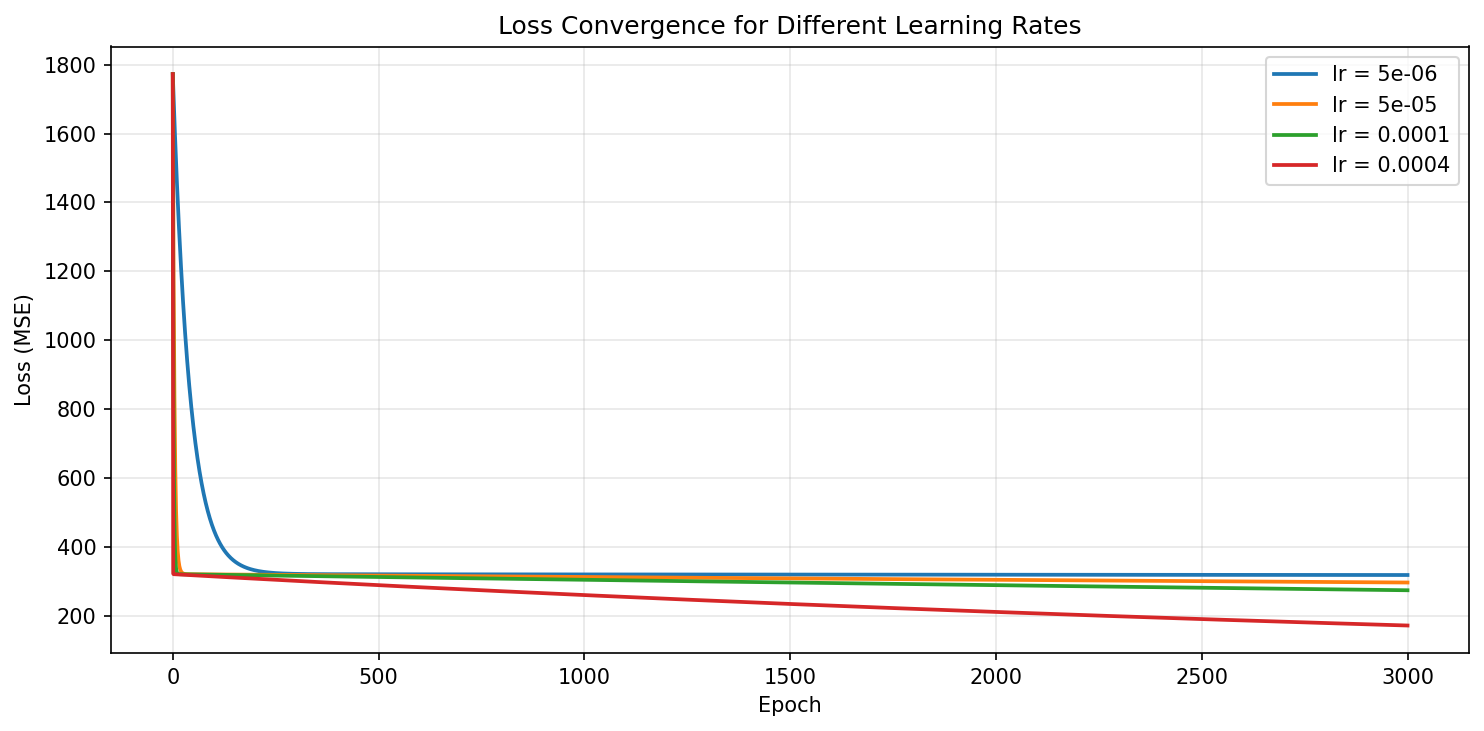
\includegraphics[width=0.85\textwidth]{loss_curves.png}
\caption{MSE loss over 3000 epochs. A larger $r$ leads to a lower final loss within the same number of epochs.}
\end{figure}

\begin{figure}[H]
\centering
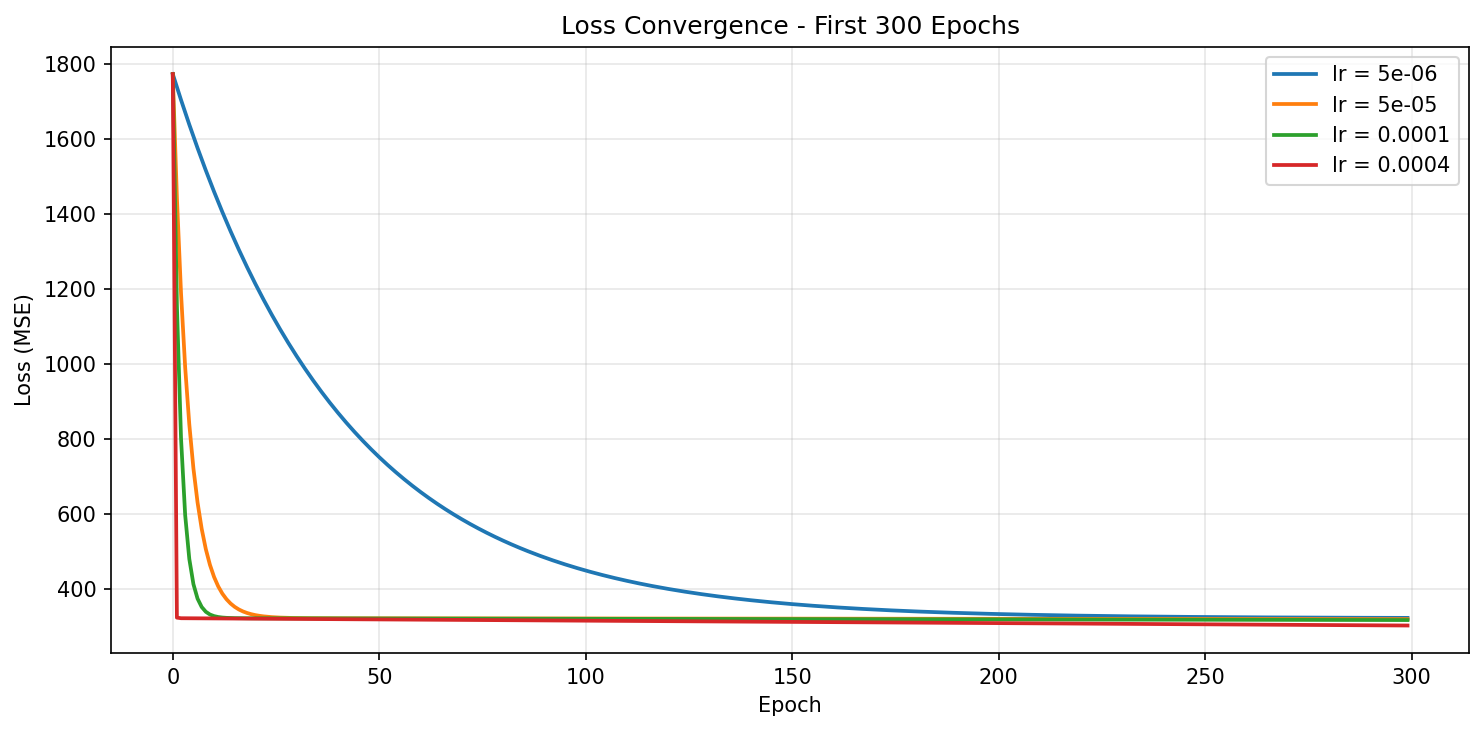
\includegraphics[width=0.85\textwidth]{loss_curves_early.png}
\caption{Loss during the first 300 epochs. Differences in convergence speed are most visible in the early phase.}
\end{figure}

\begin{figure}[H]
\centering
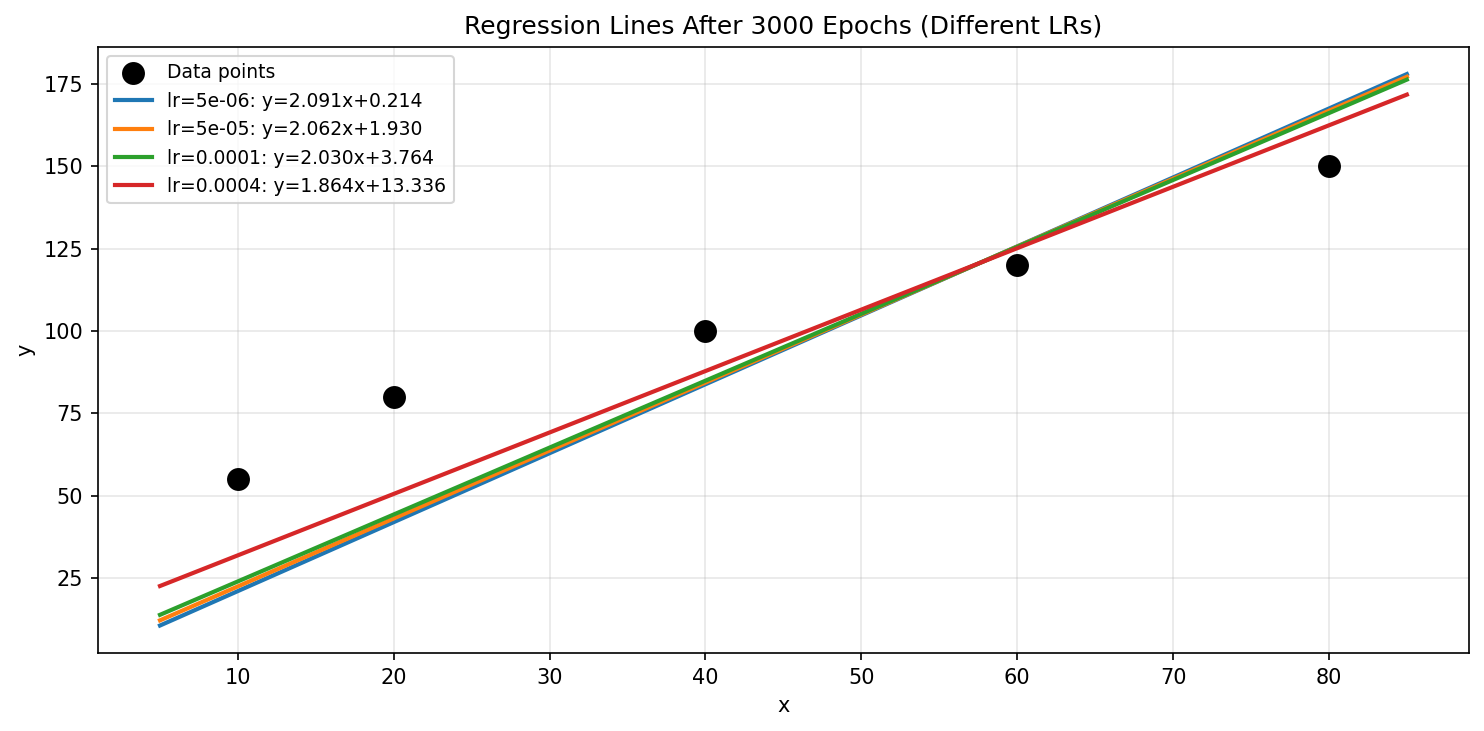
\includegraphics[width=0.85\textwidth]{regression_lines_comparison.png}
\caption{Regression lines after 3000 epochs. A larger $r$ produces a line that fits the data more closely within the same number of epochs.}
\end{figure}

\textbf{Analysis:}
\begin{itemize}
    \item \textbf{$r = 5\times10^{-6}$:} After 3000 epochs the loss is 318.8, barely lower than at epoch 10 (326.8). The model makes negligible progress per step.
    \item \textbf{$r = 5\times10^{-5}$:} Loss reaches 297.0 --- faster than above but still slow.
    \item \textbf{$r = 1\times10^{-4}$:} Loss reaches 274.5. This is the default baseline.
    \item \textbf{$r = 4\times10^{-4}$:} Loss reaches 172.2, the best result in this comparison. Larger steps allow faster descent without diverging.
    \item \textbf{Too large $r$:} If $r$ exceeds the safe bound, updates overshoot the minimum and the loss diverges.
\end{itemize}

The slow convergence across all tested rates is due to the absence of feature normalization. The $x$ values (10--80) cause the gradient of $w_1$ to be much larger than that of $w_0$, making it hard to choose a single $r$ that is ideal for both parameters at once.

\section{Conclusion}

I implemented Linear Regression from scratch using Gradient Descent in pure Python, with no numerical libraries. The algorithm correctly applies the partial derivatives of the MSE loss to update both $w_0$ and $w_1$ simultaneously. Experiments with four learning rates confirm that:
\begin{enumerate}
    \item A very small learning rate results in extremely slow convergence.
    \item Increasing the learning rate speeds up convergence, up to a limit beyond which the loss diverges.
    \item Without feature normalization, gradient descent on this dataset converges slowly because the gradient scales for $w_0$ and $w_1$ differ significantly.
\end{enumerate}

\end{document}
